
%\documentclass[manuscript]{acmart}
%\documentclass[acmsmall]{acmart}
%\settopmatter{printacmref=false}


\documentclass[
  a4paper,
  12pt,
  DIV=12,        % höherer Wert = schmalere Ränder, weniger Whitespacmi
  parskip=half,  % Absätze mit halbem Abstand statt Einzug
  headings=small % kleinere Überschriften, weniger vertikaler Abstand
]{scrartcl}

%\documentclass[a4paper,11pt]{scrartcl}
%\documentclass[a4paper,11pt]{report}
%\documentclass[a4paper,12pt]{book}
\usepackage[utf8]{inputenc}
\usepackage[german]{babel}
\usepackage[T1]{fontenc}
\usepackage{lmodern}
\usepackage[inkscapelatex=false]{svg}
% Texte im SVG von Inkscape setzen lassen, nicht durch die Dokumentschrift ersetzen
\svgsetup{inkscapelatex=false}
\usepackage{amsmath}
\usepackage{caption}
\usepackage{gensymb}
\usepackage{microtype}
\usepackage{longtable}
\usepackage{tabularx}   % Spalten, die die restliche Zeilenbreite auffüllen (X-Spalte)
\usepackage{booktabs}   % \toprule \midrule \bottomrule (in mobrob_table.tex verwendet)
\usepackage{wrapfig}    % Textumfluss um Abbildungen
\usepackage{array}
\usepackage{calc}
\usepackage{eurosym}


\usepackage[citecolor=black, colorlinks=true, linkcolor=black, urlcolor=blue]{hyperref}


%\usepackage{geometry}
\usepackage{siunitx}
%\geometry{margin=2.5cm}


\usepackage{amsthm}
\usepackage{mdframed}
\usepackage{enumitem}

\newmdtheoremenv{theorem}{Theorem}

\theoremstyle{definition}
\newmdtheoremenv{derivation}{Derivation}

\providecommand{\tightlist}{%
  \setlength{\itemsep}{0pt}\setlength{\parskip}{0pt}}

%\mdfdefinestyle{leftline}{
%    topline=false, bottomline=false, rightline=false,
%    linewidth=2pt, linecolor=gray
%}
\theoremstyle{definition}
\newmdtheoremenv[style=leftline]{myalgorithm}{Algorithm}




%\usepackage{fancyvrb}







\let\Bbbk\relax
\usepackage{amssymb}


\usepackage{yfonts}

\usepackage{kvmap}

% \usepackage[
%     backend=biber,
%     style=alphabetic,
%     sortlocale=de_DE,
%     natbib=true,
%     %url=false,
%     doi=true,
%     %eprint=false
% ]{biblatex}
% \addbibresource{Literaturrecherche-Stefan-Etringer/algo-references.bib}

%\usepackage[
%    backend=biber,
%    style=alphabetic,
%    sortlocale=de_DE,
%    natbib=true,
%    %url=false,
%    doi=true,
%    %eprint=false
%]{biblatex}
%\addbibresource{Literaturrecherche-Dennis/mobrob_references.bib}

\usepackage[autostyle=true,german=quotes]{csquotes}
\usepackage{trfsigns} %fourier transform arrow
\usepackage{mathrsfs} %fourier F
\usepackage{commath}

\usepackage{pgfplots}
\pgfplotsset{compat=1.18}

\usepackage{xcolor}
\usepackage{listings}
\usepackage[european]{circuitikz}
\ctikzset{tripoles/european not symbol=ieee circle}

%\usepackage[shading]{moeptikz}
%\moeptikzset{shading=true}

%\usepackage{german,longtable}

\usepackage{xcolor}
\usepackage{color}
\usepackage{url}

\usepackage{xfrac}

\usepackage{listings}
\usepackage{verbatimbox}

\usepackage{algorithm}
\usepackage{algpseudocode}

\usepackage{multirow}
\usepackage{float}
\usepackage{pdflscape}   % einzelne Querformatseiten (im PDF gedreht)

%%%% TIKZ

\usepackage{tikz}

\usepackage{pgfplots}
\usetikzlibrary{calc,
trees,positioning,arrows,
chains,shapes.geometric,
decorations.pathreplacing,
decorations.pathmorphing,shapes,
matrix,shapes.symbols,
plotmarks}
%\tikzexternalize[prefix=figures/]

%\tikzset{%
%  block/.style    = {draw, thick, rectangle, minimum height = 3em,
%    minimum width = 3em},
%  sum/.style      = {draw, circle, node distance = 2cm}, % Adder
%  input/.style    = {coordinate}, % Input
%  output/.style   = {coordinate} % Output
%}
% Defining string as labels of certain blocks.
%\newcommand{\suma}{\Large$+$}
%\newcommand{\multa}{\Large$\times$}
%\newcommand{\inte}{$\displaystyle \int$}
%\newcommand{\derv}{\huge$\frac{d}{dt}$}

\usetikzlibrary{arrows,automata,positioning}
%\usepackage{automata}


%%% END TIKZ

\usepackage[section]{placeins}

\usepackage{textcomp}


\usepackage{listings}
\usepackage{verbatimbox}

\usepackage{bold-extra}

\usepackage{framed}

\usepackage[table]{xcolor}

%\usepackage{fancyhdr}
%\pagestyle{fancy}
%\lhead{\leftmark}
%\chead{}
%\rhead{}
%\lfoot{}
%\cfoot{\thepage}
%\rfoot{}
%\renewcommand{\headrulewidth}{0.2pt}
%\renewcommand{\footrulewidth}{0.2pt}



\newcommand{\Z}{\mathbb{Z}}
\newcommand{\R}{\mathbb{R}}
\newcommand{\C}{\mathbb{C}}
\newcommand{\N}{\mathbb{N}}
\newcommand{\SqrtNy}{$\sqrt{\textsc{Ny}}$}
\newcommand{\conj}{\overline}
\newcommand{\Kset}{\textswab{K}}
\newcommand{\Qset}{\textswab{Q}}
\newcommand{\ceil}[1]{\left\lceil #1 \right\rceil}
\newcommand{\floor}[1]{\left\lfloor #1 \right\rfloor}
\newcommand{\sorted}[1]{\textsc{sort}\left\lbrace #1 \right\rbrace}
\newcommand{\SNRgain}{a_{SNR}}
\newcommand{\EQgain}{a_{EQ}}
\newcommand{\SIRgain}{a_{SIR}}
\newcommand{\SNIRgain}{a_{SINR}}
\newcommand{\SNR}{\textsc{SNR}}
\newcommand{\CIRgain}{a_{CIR}}
\newcommand{\CINRgain}{a_{CINR}}
\newcommand{\CNR}{\textsc{CNR}}
\newcommand{\CINR}{\textsc{CINR}}
\newcommand{\HPAModel}{ Hughes 1177H TWTA }
\newcommand{\bigO}{\mathcal{O}}
\newcommand{\CopWinCompl}{2.375377}
\newcommand{\IBO}{\textsc{IBO}}
\newcommand{\OBO}{\textsc{OBO}}
\newcommand{\spacepage}{\newpage\null\thispagestyle{empty}\newpage}
\newcommand{\satcom}{ SatCom }
\newcommand{\db}{~\text{dB}}


\definecolor{mGreen}{rgb}{0,0.6,0}
\definecolor{mGray}{rgb}{0.5,0.5,0.5}
\definecolor{mPurple}{rgb}{0.58,0,0.82}
\definecolor{backgroundColour}{rgb}{0.95,0.95,0.92}

\lstdefinestyle{CStyle}{
    backgroundcolor=\color{backgroundColour},
    commentstyle=\color{mGreen},
    keywordstyle=\color{magenta},
    numberstyle=\tiny\color{mGray},
    stringstyle=\color{mPurple},
    basicstyle=\footnotesize,
    breakatwhitespace=false,
    breaklines=true,
    captionpos=b,
    keepspaces=true,
    numbers=left,
    numbersep=5pt,
    showspaces=false,
    showstringspaces=false,
    showtabs=false,
    tabsize=2,
    language=C
}

\lstdefinelanguage{VHDL}{
  morekeywords=[1]{library,use,all,entity,is,port,in,out,end,architecture,of,begin,process,if,then,else,elsif,when,others,signal,variable,wait,for,loop},
  morecomment=[l]--,
  morestring=[b]",
  sensitive=true
}

\lstset{
  language=VHDL,
  basicstyle=\ttfamily\small,
  keywordstyle=\color{blue},
  commentstyle=\color{gray},
  stringstyle=\color{red},
  numbers=left,
  numberstyle=\tiny,
  stepnumber=1,
  numbersep=8pt,
  frame=single,
  breaklines=true,
  captionpos=b
}

\lstset{numbers=none}

%\newcounter{example}
%\renewcommand{\theexample}{\thesection.\arabic{example}}


% Default fixed font does not support bold face
\DeclareFixedFont{\ttb}{T1}{txtt}{bx}{n}{12} % for bold
\DeclareFixedFont{\ttm}{T1}{txtt}{m}{n}{12}  % for normal

% Custom colors
\usepackage{color}
\definecolor{deepblue}{rgb}{0,0,0.5}
\definecolor{deepred}{rgb}{0.6,0,0}
\definecolor{deepgreen}{rgb}{0,0.5,0}

\usepackage{listings}

% Python style for highlighting
\newcommand\pythonstyle{\lstset{
language=Python,
basicstyle=\ttm,
morekeywords={self},              % Add keywords here
keywordstyle=\ttb\color{deepblue},
emph={MyClass,__init__},          % Custom highlighting
emphstyle=\ttb\color{deepred},    % Custom highlighting style
stringstyle=\color{deepgreen},
frame=tb,                         % Any extra options here
showstringspaces=false
}}


% Python environment
\lstnewenvironment{python}[1][]
{
\pythonstyle
\lstset{#1}
}
{}

% Python for external files
\newcommand\pythonexternal[2][]{{
\pythonstyle
\lstinputlisting[#1]{#2}}}

% Python for inline
\newcommand\pythoninline[1]{{\pythonstyle\lstinline!#1!}}


% ---------------------------------------------------------------------
% Stil fuer C++-Listings dieser Dokumentation
% ---------------------------------------------------------------------
\lstdefinestyle{cpp}{
  language=C++,
  basicstyle=\ttfamily\footnotesize,
  keywordstyle=\color{deepblue},
  commentstyle=\color{mGreen},
  stringstyle=\color{mPurple},
  numbers=none,
  breaklines=true,
  showstringspaces=false,
  frame=single,
  columns=fullflexible,
  captionpos=b
}



%\nocite{*}


\begin{document}
%\pagenumbering{roman}




\title{Konzeptionieren eines Coasterbots}
\subtitle{Endbericht}
\author{Dennis Borutta, Stefan Etringer, Gereon Such}
%\email{gereonsuch@suchdsp.com}
%\affiliation{
%  \institution{Wilhelm Büchner University of Applied Sciences}
%  \department{Computer Engineering}
%  \city{Hof}
%  \country{Germany}
%}



\begin{titlepage}
  \begin{center}
    {\large Wilhelm Büchner University of Applied Sciences} \\[0.3em]
    
    {\normalsize Projektarbeit Master}
\vspace{5em}

    {\LARGE\bfseries Thema: \\[0.5em] Konzeptionieren eines Coasterbots} \\[2em]

    {\large Endbericht} \\[2em]

    {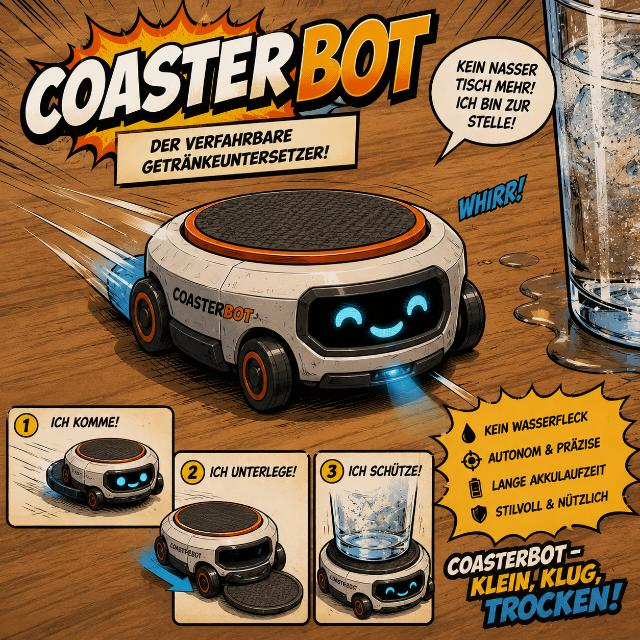
\includegraphics[width=0.38\textwidth]{coasterbot.png}} \\[1em]

\vspace{4em}

    {\normalsize
\begin{tabular}{c}
  \textbf{Team: Coasterbot}
\end{tabular}
    }

    {\normalsize
\begin{tabular}{ll}
\textbf{Studierender} & \textbf{Matrikelnummer}\\
Dennis Borutta, B. Eng & 857962\\
Stefan Etringer, B. Eng & 865769\\
Gereon Such, M. Sc. & 867070\\
\end{tabular}
    }

\vspace{4em}

\begin{tabular}{lllll}
  \textbf{Betreuer:} & Dr.-Ing. Winfried Tiedge & \hspace{1em} 
  & \textbf{Abgabedatum:} & 07.11.2026
\end{tabular}

  \end{center}


\end{titlepage}


% einleitung preambel etc.


% Versionshistorie des Dokuments: eigene Seite direkt nach dem Titelblatt
\section*{Versionshistorie}
\begin{tabularx}{\textwidth}{@{}clp{2.6cm}X@{}}
\toprule
\textbf{Version} & \textbf{Datum} & \textbf{Bearbeiter} & \textbf{Änderungen}\\
\midrule
1 & 25.09.2026 & Borutta & Erster Entwurf.\\
2 & 08.10.2026 & Such & Erstfassung eigener Anteile.\\
\bottomrule
\end{tabularx}

\newpage

\tableofcontents

\newpage

% =====================================================================
\section{Einleitung}\label{einleitung}
% =====================================================================

\section{Projektumsetzung}\label{projektumsetzung}
Planumfang ca. 9 Seiten
Davon: Dennis 3 Seiten, Stefan 3 Seiten, Gereon 3 Seiten
\subsection{Projektziel (Dennis Borutta)}\label{projektziel}
Inhalt ca 0,5 Seiten

\subsection{Lösungsweg: Mechanischer Aufbau (Dennis Borutta)}\label{lösungsweg-mechink}
Inhalt ca 1 Seite
\begin{itemize}
    \item Erarbeitung des Lösungsweges: Benchmarking, Abgrenzung Ihres Vorgehens und der Wahl der Mittel von alternativen Lösungsmöglichkeiten, Begründung Ihres Ansatzes
\end{itemize}
\subsection{Lösungsweg: Algorithmik und Simulation (Stefan Etringer)}\label{lösungsweg-algorithmik}
Inhalt ca 2 Seiten
\begin{itemize}
    \item Erarbeitung des Lösungsweges: Benchmarking, Abgrenzung Ihres Vorgehens und der Wahl der Mittel von alternativen Lösungsmöglichkeiten, Begründung Ihres Ansatzes
\end{itemize}
\subsection{Lösungsweg: Elektronik und Abstraktion (Gereon Such)}\label{lösungsweg-elektronik}
Inhalt ca 2 Seiten
\begin{itemize}
    \item Erarbeitung des Lösungsweges: Benchmarking, Abgrenzung Ihres Vorgehens und der Wahl der Mittel von alternativen Lösungsmöglichkeiten, Begründung Ihres Ansatzes
\end{itemize}



\subsubsection*{Ausgangslage und Leitlinien}


Die im Pflichtenheft definierten Hardwarefunktionen mussten durch entsprechende Sensorik, Aktorik und Rechenleistung abgedeckt werden:
\begin{itemize}
\item \texttt{HW-CPU-001..004} Rechenleistung für Sensordatenverarbeitung und Navigation
\item \texttt{HW-SEN-001..005} Hindernis und Tischkantenerkennung
\item \texttt{HW-SEN-006/007} Positionierung und Orientierung
\item \texttt{HW-ACT-001..004} Bewegungssteuerung
\item \texttt{HW-ACT-005..007} Untersetzeraufnahme und -ausgabe
\item \texttt{HW-PWR-*} Energieversorgung
\end{itemize}

Ein weiteres Kriterium bei der Komponentenauswahl war schnelle und problemlose Verfügbarkeit in geringen Stückzahlen sowie ein geringer Preis. Da eine PCB Fertigung inklusive Versand einen enormen Zeitaufwand impliziert, z.B. JLCPCB ca. 4 Wochen, wurden alle Komponenten als Development-Boards beschafft und diese auf Lochrasterplatine sowie mit Steckverbindern auf Pinheadern verbunden. Jede Komponente wurde iterativ in Betrieb genommen und die Funktionalität sowie Eignung einzeln verifiziert. Dabei ergeben sich in einzelnen Fällen Schwierigkeiten, die Anpassungen erforderten, dies soll im Anschluss an die ursprüngliche Auswahl der Komponenten erläutert werden. 



\subsubsection*{Benchmarking und Auswahl der Komponenten}

Die Auswahl der Komponenten wurde in Phase M3 (Alternativenbeschreibung) diskutiert, hier wurden für jede Anforderung Lösungsvarianten identifziert und eine ausgewählt. Tabelle \ref{tab:elektronik-auswahl} fasst die wesentlichen Entscheidungen zusammen.

\begin{table}[H]
\centering
\footnotesize
\caption{Betrachtete Alternativen und gewählte Lösung der Elektronik.}
\label{tab:elektronik-auswahl}
\begin{tabularx}{\textwidth}{@{}>{\raggedright\arraybackslash}p{2.1cm}>{\raggedright\arraybackslash}p{3.1cm}>{\raggedright\arraybackslash}p{2.9cm}X@{}}
\toprule
\textbf{Funktion} & \textbf{Alternativen} & \textbf{Gewählt} & \textbf{Begründung}\\
\midrule
Controller & Arduino Uno, ESP32, Raspberry Pi Pico2 & Raspberry Pi Pico~2 (RP2350) &
Uno nicht performant genug. Pico2 nimmt weniger Leistung auf als ESP32 und hat mit PIO Interface Möglichkeit zeitkritische Signale zu generieren. \\
\midrule
Hindernis\-erkennung & Ultraschall HC-SR04, Kamera OV7670, Bumper, IR-Sensor &
HC-SR04 in Fahrtrichtung &
Unfälle auf dem Tisch sind zu wahrscheinlich mit Bumper Sensor. HC-SR04 bietet einfache und günstige Distanzmessung ohne Bildverarbeitung. Die Kamera wurde wegen des Verarbeitungsaufwands auf dem Mikrocontroller zurückgestellt.\\
\midrule
Tischkanten\-erkennung & IR-Reflexsensor, Kamera & 4 IR-Sensormodule (je Ecke) & Kamera zurückgestellt, daher alternativlos. \\
\midrule
Lage und Odometrie & IMU, Radencoder, Kamera & MPU-6050 (I$^2$C) und LM393-Gabel\-lichtschranken &
Die IMU (Inertialsystem) liefert die Drehung, die Encoder die gefahrene Strecke. Die Radencoder wurden während der Testphase ergänzt (siehe unten).\\
\midrule
Untersetzer\-mechanik & Micro-Servo, Schrittmotor & 2 Micro-Servos (MG90) & Positionsgeregelt, nur ein Signalpin, aufgrund hohen Widerstands des PETG Aufbaus mussten Metallgewinde gewählt werden.\\
\midrule
Antrieb & TT-Motoren mit H-Brücke & 4 TT-Motoren (1:48), 2$\times$ TB6612FNG &
Günstig und als Set mit Rädern verfügbar. Der Regler TB6612FNG wurde aufgrund geringerer Verlustleistung als der L298N gewählt.\\
\midrule
Energie\-versorgung & 9-V-Block mit Linearregler 78x05; Li-Ion-Akku mit DC/DC-Wandler &
18650-Li-Ion-Akku (\SI{3.7}{\volt}) mit Step-Up-Wandler auf \SI{5}{\volt} &
Die gewählten Motoren bedürfen recht hoher Ströme, dieser kann nicht durck Linearregler geliefert werden. Folglich Motorspannung \texttt{VM} direkt am Akku, Steuerspannung \texttt{VCC} über Step-Up-Wandler. \\
\midrule
Bedienung und Status & RGB-LED oder diskrete LEDs; Taster & RGB-LED, Taster, Hauptschalter & Eine RGB-LED kann alle Betriebszustände über Farbe und Blinkmuster darstellen.\\
\bottomrule
\end{tabularx}
\end{table}

\subsubsection*{Elektrischer Aufbau}

Die Schaltung wurde in der Open Source Software KiCad erstellt (Abbildung~\ref{fig:endbericht-schematic}) und mit der Software DIYLC auf ein Lochrasterplatinenlayout im Raster $30 \times 24$ übertragen. Externe Komponenten werden über Pin Header angeschlossen. Die Platine trägt den Mikrocontroller, den Step-Up-Wandler, die
Motortreiber, das Inertialsystem, die RGB-LED, Glättungskondensatoren für die Versorgungsspannungen sowie Pulldown Widerstand und Endprellung für den Taster. Der Aufbau ist in der Aufbauanleitung (M4) detailliert dokumentiert.

\begin{figure}[H]
  \centering
  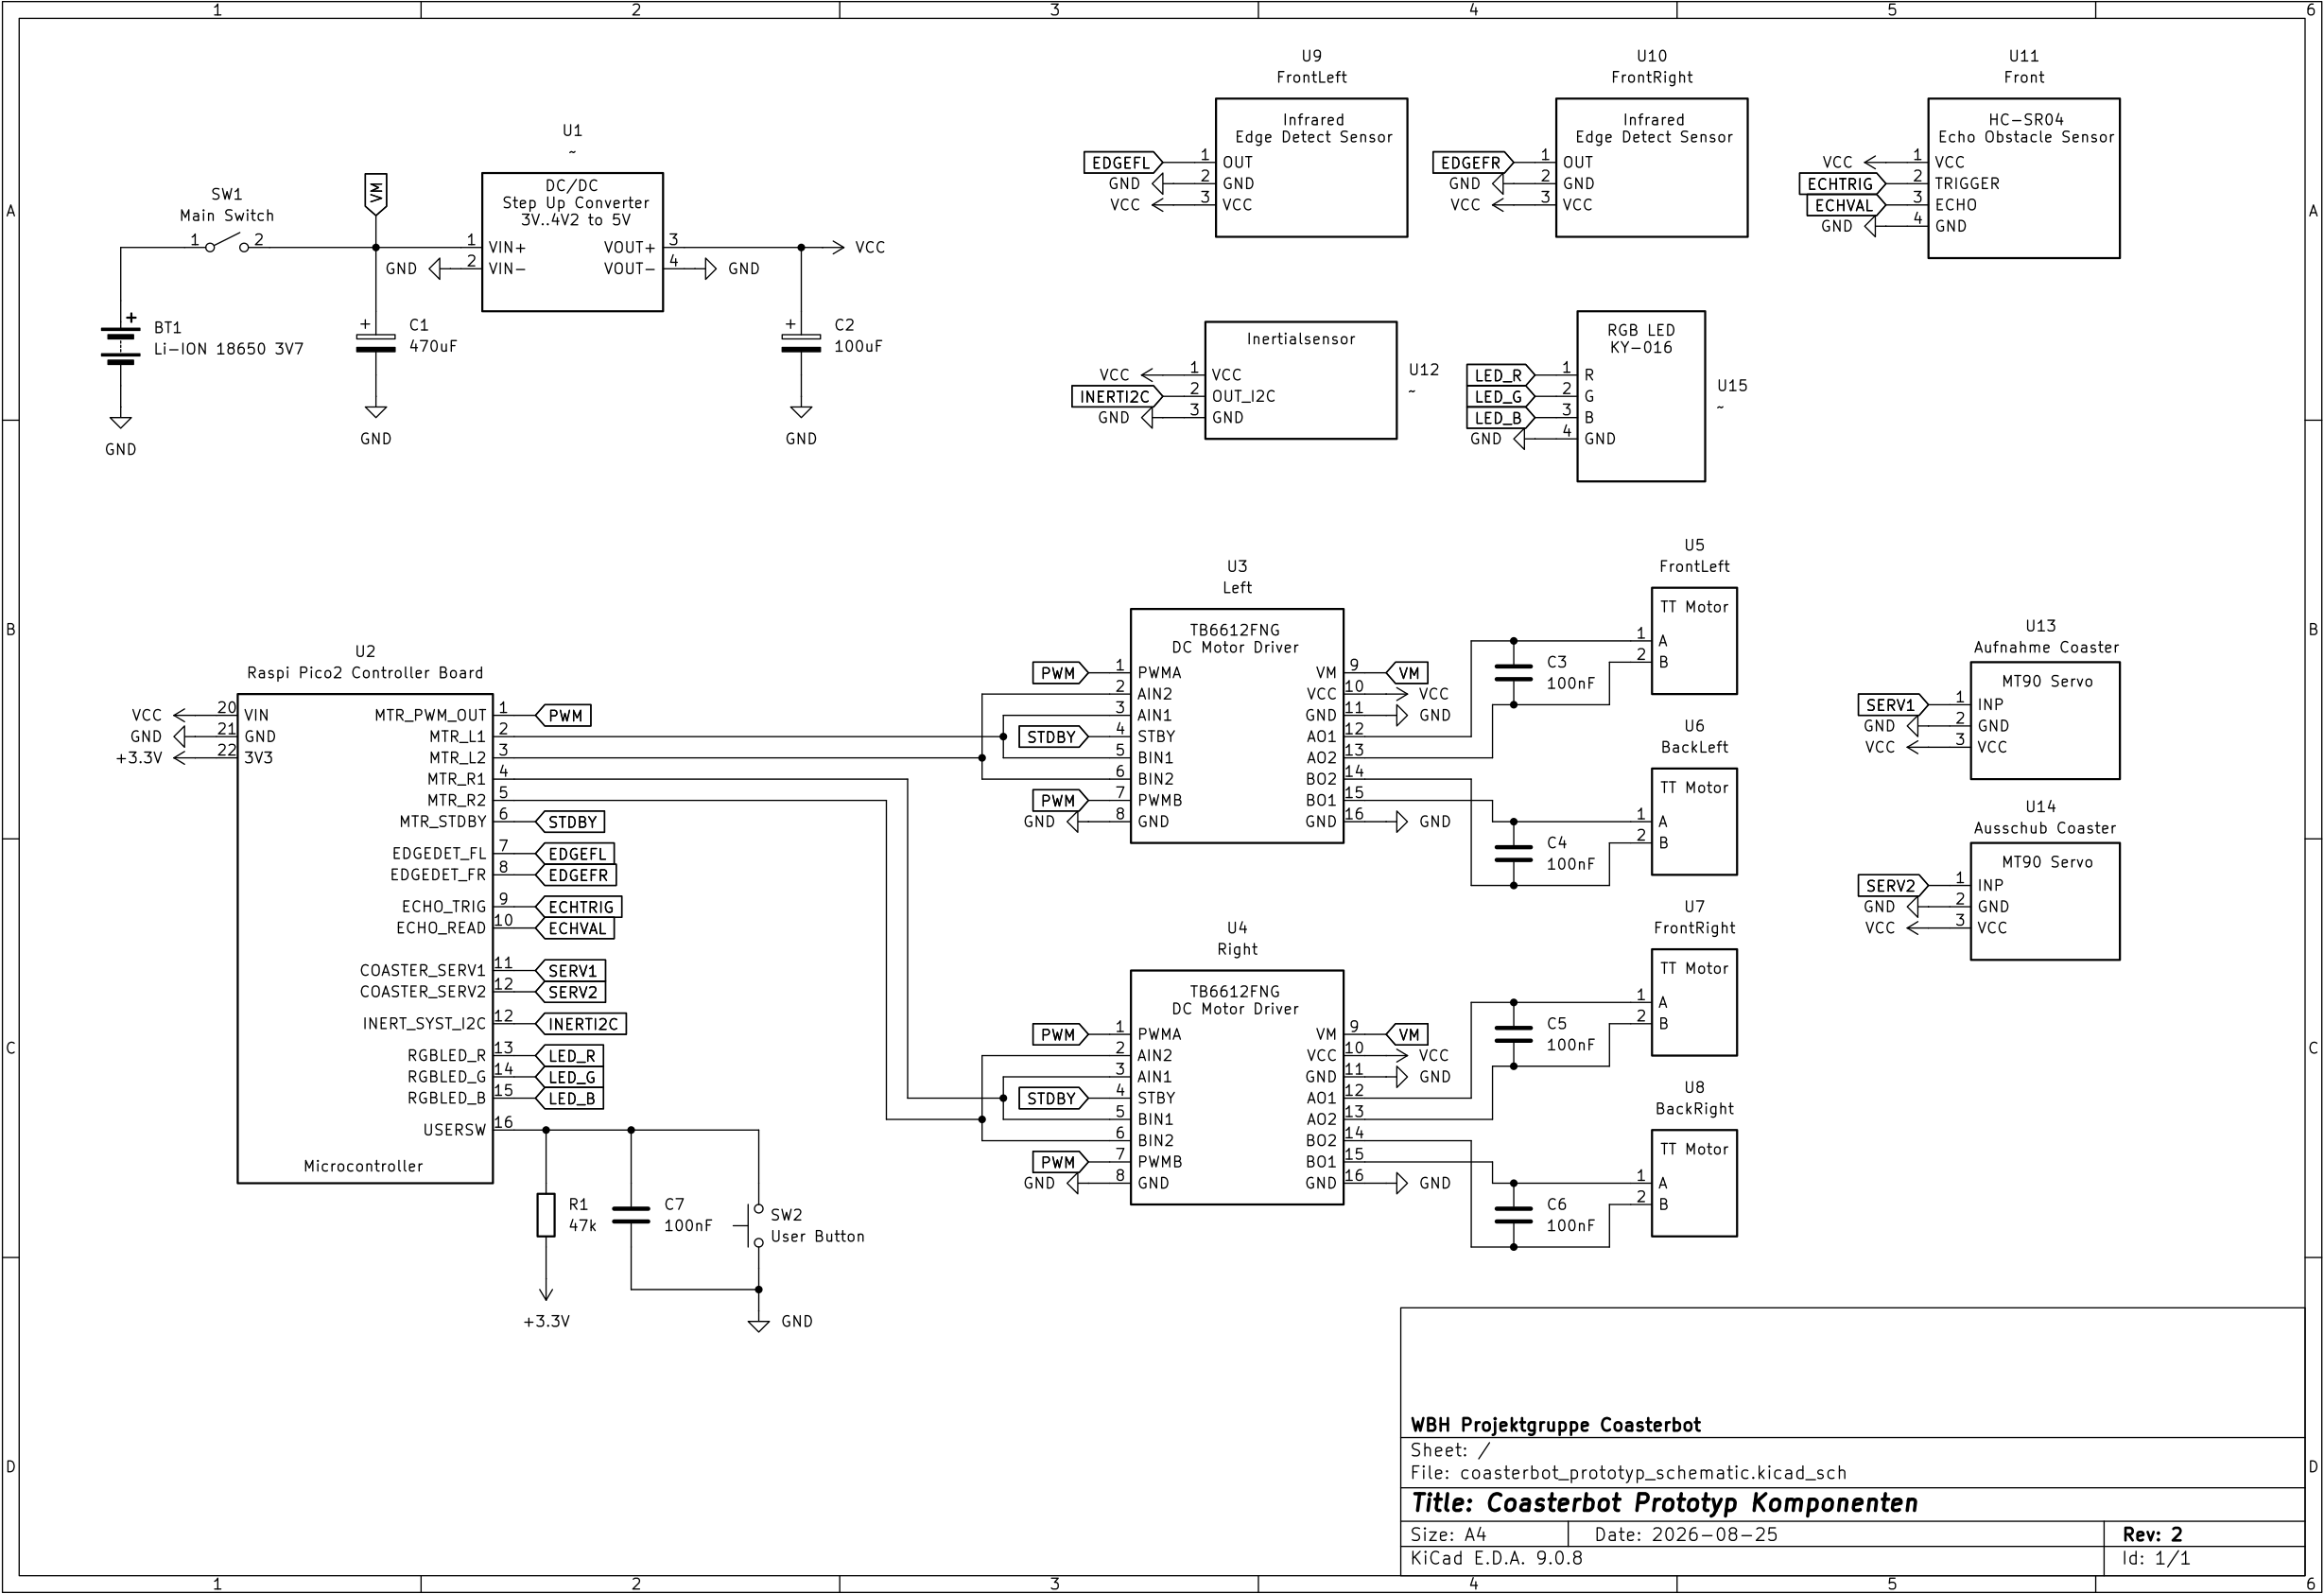
\includegraphics[width=\textwidth]{../M4_Test-und-Validierung/aufbauanleitung/schematic.png}
  \caption{Gesamtschaltung der Elektronik (aus der Aufbauanleitung).}
  \label{fig:endbericht-schematic}
\end{figure}

Beide Motoren einer Seite sind durch je einen Motortreiber geregelt, wobei sich beide Motortreiber das Standby- sowie PWM-Signal teilen. Dadurch drehen alle Motoren stets betragsmäßig gleich schnell. In der Folge sind nur Geradeausfahrt vorwärts/rückwärts als auch bei entgegengesetzter Drehrichtung Kurven auf der Stelle möglich. Diese Vereinfachung kann für eine zukünftige Ausbaustufe eventuell überdacht werden, da die Positionserkennung durch Odometrie(Zählen der Rad-Rotationen) bei Rotation auf der Stelle verhätnismßig ungenau ausfällt. Dies ergab sich in den Inbetriebnahmetests und wurde durch das Intertialsystem kompensiert. 


\subsubsection*{Hardwareabstraktion}

Die zentrale Schnittstelle ist die abstrakte C++-Klasse \texttt{RobotHAL}, die in der Simulation parallel zur Entwicklung der Elektronik definiert wurde. Sie beschreibt die Fähigkeiteiten des Roboters(Geschwindigkeit je Seite, Objektdistanz nach vorne, Kantensensor, Drehrate, Encoderwinkel, Zeit, Servosteuerung und LED), und referenziert weder die Webots Implementierung noch die eigentlichen Hardwareimplementierungen. Diese abstrakte Basisklasse wird dann in der \texttt{HardwareImplementationHAL} implementiert und bindet dann die Controller der einzelnen Komponenten ein. Diese Controller sind im Projekt Source Code als Template Klassen für die Hardwareparameter auf dem Arduino Framework implementiert. In der Hardwareabstraktion werden dann alle Controller mit den entsprechenden Pins aus einer Projektkonfigurationsdatei instanziiert und kombiniert. 

Alle Komponenten sind \textit{non-blocking} implementiert. Wenn z.B. die Motorsteuerung einer Seite sich derzeit in Vorwärtsdrehung befindet, dann durch die Steuerung aber ein Richtungswechsel ausgelöst wird, so muss zunächst aktiv abgebremst werden und erst wenn dieser Bremsvorgang beendet ist darf der Motor wieder in Rückwärtsrichtung angesteuert werden. Solche zeitabhängigen Vorgänge können natürlich durch \texttt{delay}/\texttt{sleep}-Befehle gelöst werden, in dieser Zeit erfolgt aber auch keine Sensorauswertung oder weitere Parametrierungen. Der Non-blocking Ansatz implementiert in den Komponenten jeweils eine interne Statemachine, die nach variablen Zeitintervallen einen Zustandsübergang durchführt und die Ausgangssignale anpasst oder nur in fixen Zeitintervallen Sensorwerte wiederum ausliest. Alle Aktionen finden in der Anwendungslogik weiterhin seriell statt, aber in geplanten Intervallen in \texttt{step} oder \texttt{update} Methoden, die in jedem Hauptschleifenzyklus durchlaufen werden und meistens direkt zurückspringen (Early Exit). 

\subsubsection*{Anpassungen während der Umsetzung}

Der ursprüngliche Ansatz für das Positionierungssystem war eine Integration des Beschleunigungssensors um einen Geschwindigkeitswert zu erhalten, Da die TT Motoren eine solche Information schlicht nicht bereitstellen können. Dieser Geschwindigkeitswert sollte wiederum integriert werden um eine absolute Positionierung zu erhalten. 

Während der Hardwaretests zeigte sich, dass trotz Bias-Kalibrierung, Lagekorrektur und Stillstandserkennung in Verbindung mit der Motorsteuerung die erreichbare Genauigkeit für ein Positionssystem außerhalb akzeptabler Toleranz lag: Durch Testfahrten immer wieder vorwärts und rückwärts summierte sich ein Fehler auf die aktuelle Position von einigen Dezimetern mit steigender Tendenz. In der Folge wurde die Motorhalterung modifiziert und an der dem Rad abgewandten Seite zweier TT Motoren eine Gabellichtschranke mit 20-Loch Drehscheibe und LM393 Komparator angebracht. Durch diese Kodierung ist die Änderung des Radwinkels mit $\sfrac{1}{40}$ des Umfangs bestimmbar, bei Raddurchmesser von $66$ Millimeter ergibt sich bei einem \textit{Tick} am Sensor(Wert-Wechsel) eine Fahrtstrecke von $66 \times \sfrac{\pi}{40} = 5.2$ Millimeter. Dies ist für eine gemessene Strecke zwar noch akzeptabel, aber bei Rotation wiederum zu ungenau um einen echten Drehwinkel für ein Navigationssystem zu bestimmen, weshalb der Drehwinkel weiterhin durch das IMU-System bezogen wird, wo Rotationswinkel weniger fehlerbehaftet sind als lineare Beschleunigungen. Bei der Implementierung der Tick-Erkennung wurde zusätzlich noch mit einem Hardwareinterrupt gearbeitet und konsekutive Ticks aufsummiert um sicherzustellen, dass nicht durch zu geringe Hauptschleifenfrequenz Ticks verloren gehen. Zudem wurden beide dieser Odometriecontroller mit der Motorsteuerung gekoppelt, sodass die Drehrichtung des jeweiligen Rades berücksichtigt wurde. 

Weitergehend wurde festgestellt, dass eine Drehbewegung auf der Stelle ein deutlich höheres Drehmoment im Gegensatz zu Geradeausfahrt bedarf. Dies wurde in der Motorsteuerung berücksichtigt, allerdings ist der Schlupf der Räder auf einer Tischoberfläche hier sehr hoch. Vermutlich ist also in der Folge eine Navigation mit \textit{sanften Kurven} doch zweckmäßiger. Dies sollte für eine weitere Ausbaustufe wie bereits erwähnt in Betracht gezogen werden. 

Derzeit noch nicht umgesetzt sind die Akkuüberwachung (\texttt{HW-PWR-002/003}) sowie eine Rückkopplung von Odometriesystem zu Motorsteuerung um eine tatsächliche Geschwindigkeitsregelung auf $\frac{m}{s}$ zu erreichen. Die Ansteuerung der Motoren erfolgt über das PWM Signal, das lediglich von $0$ für minimalem bis $255$ für maximales Drehmoment parametriert werden kann, die tatsächliche Drehgeschwindigkeit ist aber dann wiederum von der Motorspannung \texttt{VM} abhängig. 





\subsection{Projektergebnis (Dennis Borutta)}\label{projektergebnis}
Inhalt ca 0,5 Seiten

\subsection{Zeitplan Soll/Ist (Dennis Borutta)}\label{zeitplan-sollist}
Inhalt ca 1 Seite

\subsection{Kosten- und Ressourcenplan Soll/Ist (Gereon Such)}\label{kosten-und-ressourcenplan-sollist}
Inhalt ca 1 Seite

\subsection{Nutzen und Weiterentwicklung des Ergenis (Stefan Etringer)}\label{nutzen-des-aktuellen-ergebnis}
Inhalt ca 1 Seite

\section{Projektablauf}\label{projektablauf}
Planumfang ca. 9 Seiten
Davon: Dennis 3 Seiten, Stefan 3 Seiten, Gereon 3 Seiten


\subsection{Teambildung und Rollenverteilung (Dennis Borutta)}\label{teambildung-und-rollenverteilung}
ca 1 Seite
\begin{itemize}
    \item Wie war die Teambildung für das Projekt?
        \begin{itemize}
            \item Kurzes objektives resüme aus dem Projektstart
        \end{itemize}
    \item Wie fand die Rollenverteilung statt?
        \begin{itemize}
            \item Kurzes objektives resüme aus dem Projektstart
        \end{itemize}
\end{itemize}

\subsection{Zusammenarbeit im Projekt (Stefan Etringer)}\label{zusammenarbeit-projekt}
ca 1 Seiten
\begin{itemize}
    \item Darstellung und Bewertung der Zusammenarbeit im Projektteam
    \item Objektive Beschreibung. Bewertung später.
    \item Gitlab, DMS, Notion
\end{itemize}

\subsection{Kommunikation im Projekt (Gereon Such)}\label{kommunikation-projekt}

\textbf{Kommunikation Gereon Such:}
ca 1 Seite
\begin{itemize}
    \item Darstellung und Bewertung der Kommunikation im Projekt
    \item Objektive Beschreibung. Bewertung später.
    \item WhatsApp, Alfaview, Notion
    \item Darstellung und Bewertung der aufgetretenen Probleme bzgl. Teamarbeit und Kommunikation; Lösung dieser Probleme
    \item Objektive Beschreibung. Bewertung später.
\end{itemize}


\begin{wrapfigure}{r}{0.2\textwidth}
  \centering
  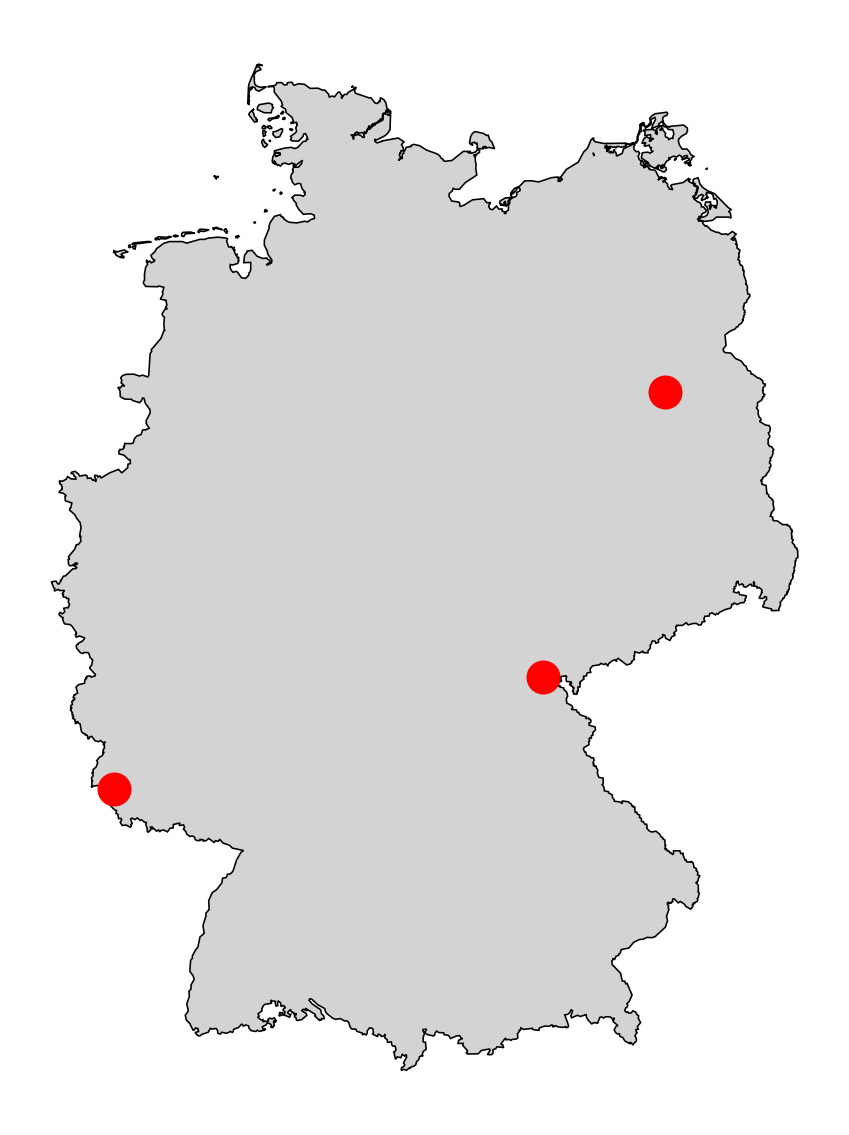
\includegraphics[width=0.18\textwidth]{deutschlandkarte.png}
\end{wrapfigure}

Das Coasterbot Team ist bei Stichprobengröße $N=3$ in guter Näherung über ganz Deutschland verteilt und die Kommunikation fand folglich komplett digital statt. Die Teamleitung und Kommunikation in den Meilensteingesprächen wurde durch Dennis Borutta wahrgenommen. Die Aufgaben wurden in Arbeitspakete auf- und im Team verteilt. Ein wöchentliches Meeting wurde per Videokonferenz durchgeführt, in denen jedes Teammitglied Fortschritte mitgeteilt, auf eventuelle Probleme hingewiesen sowie um eventuelle Hilfe gebeten hat. Kurze Rückmeldungen dazwischen wurden in der Woche über eine WhatsApp-Gruppe geteilt. In der Kommunikation traten keine Probleme auf. 


\subsubsection*{Projektverwaltung: Notion}

\begin{wrapfigure}{r}{0.6\textwidth}
  \centering
  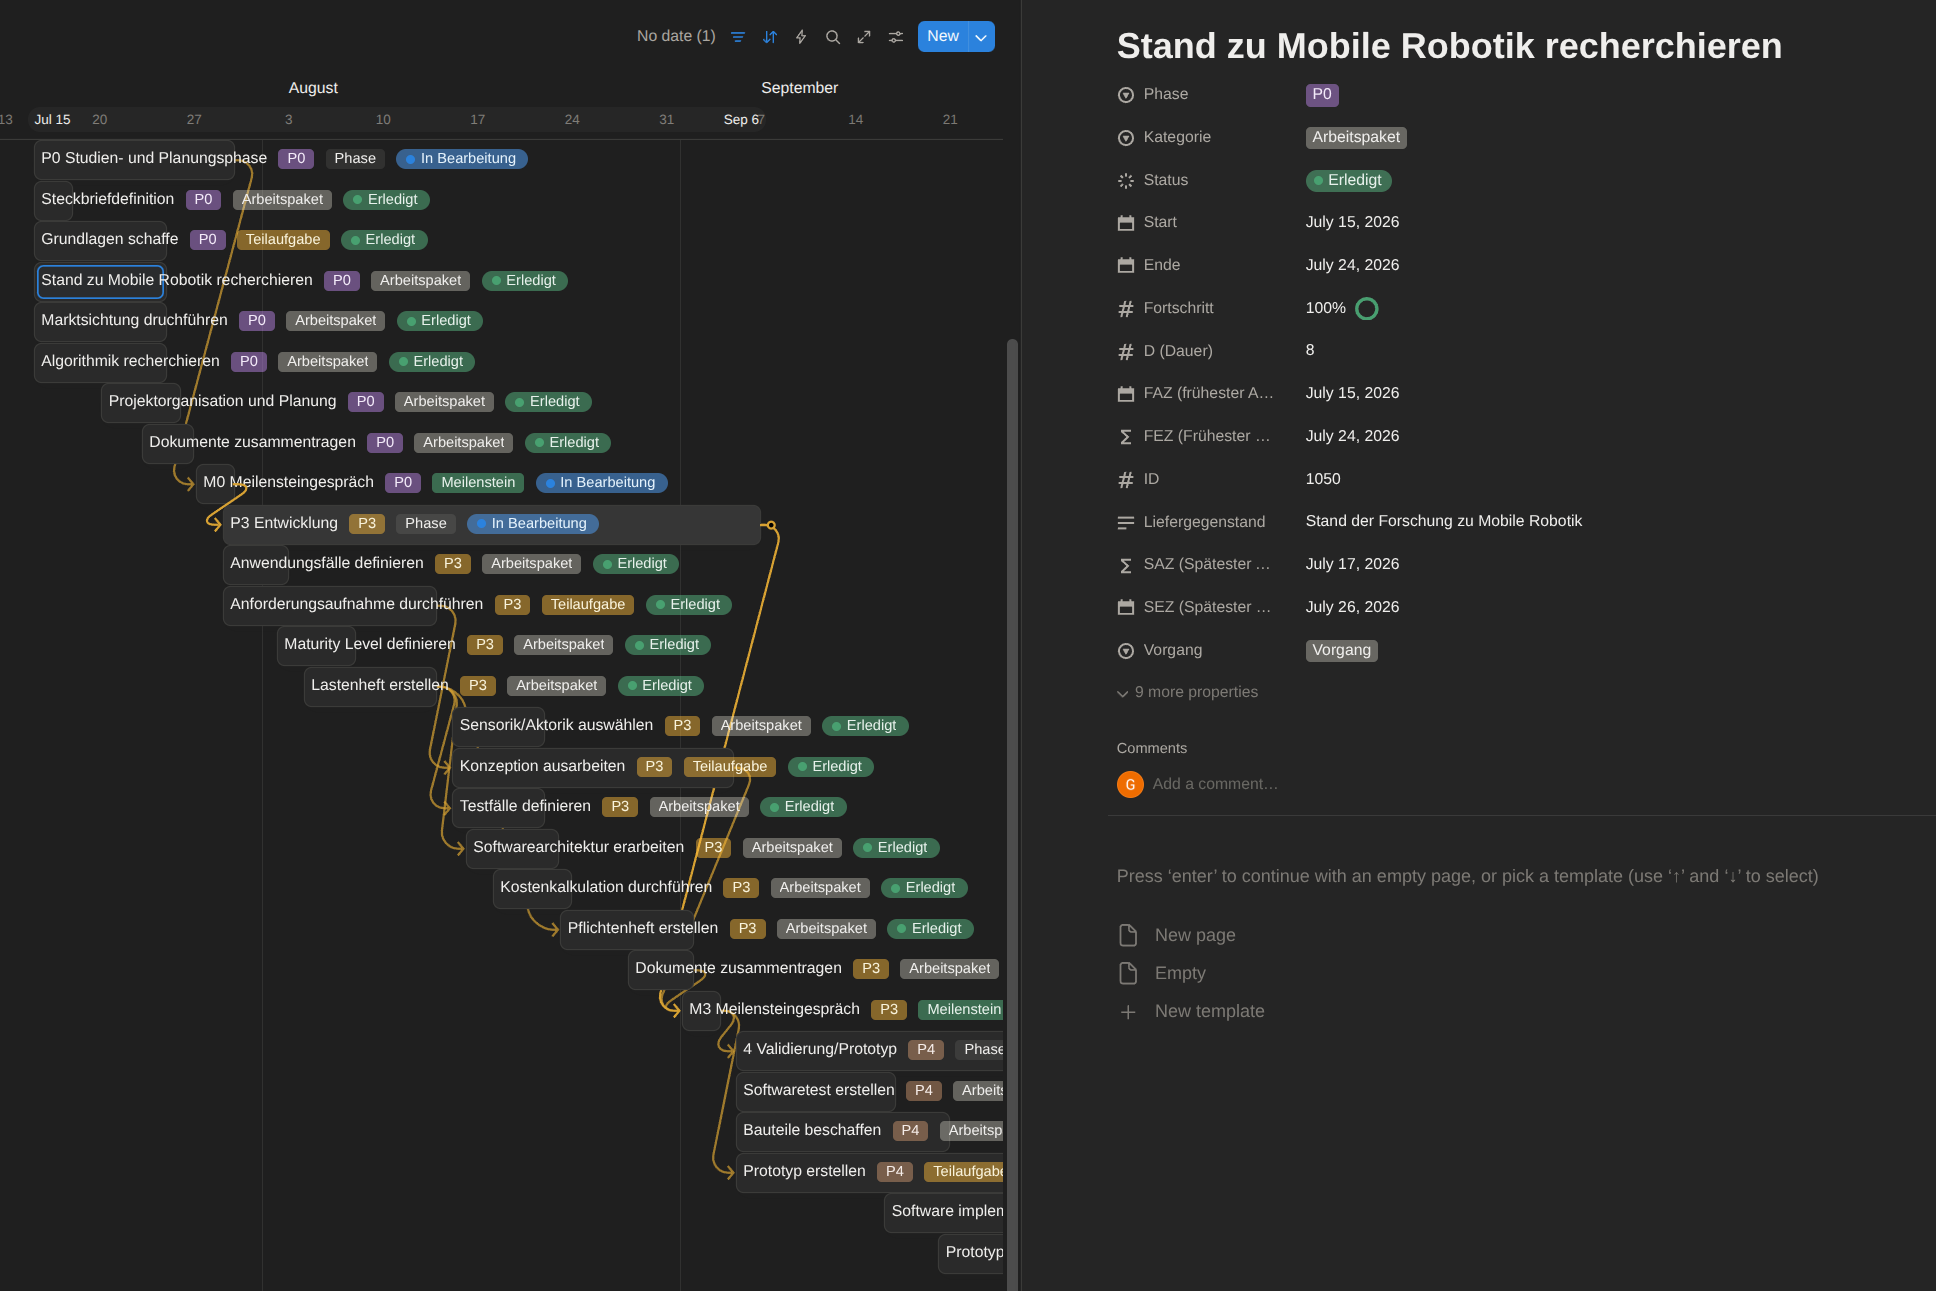
\includegraphics[width=0.58\textwidth]{notion_screenshot.png}
\end{wrapfigure}

Das Zentrale Projektsteuerungstool war \textbf{Notion}\footnote{\url{https://www.notion.com}}. Dieses wurde zur Bestimmung von Verantwortlichkeiten, Unteraufgaben, Deadlines und Terminen genutzt, hauptsächlich gepflegt durch Dennis Borutta. Es ermöglicht neben einer wie der rechts dargestellten Timelinedarstellung auch ein kollaboratives Dokumentenmanagement, welches durch das Team insbesondere in der Anfangsphase des Projekts für Recherche und Brainstorming genutzt wurde. 


\subsubsection*{Kollaborationsplatform: Github}

Das Projekt inklusive aller in \LaTeX\, erstellten Dokumente, Sourcecode und anderer Entwicklungsdateien sind in einem Github\footnote{\url{https://github.com}} Projekt verfügbar\footnote{\url{https://github.com/Project-CoasterBot/coasterbot}}. Git\footnote{\url{https://git-scm.com}} ist ein Versionsverwaltungssystem für das dezentrale Verwalten verschiedener Versionsstände und ist für das Coasterbot Projekt gewählt worden weil das Team bereits vertraut mit diesem Tool war, es kostenlos und Cross-Platform verfügbar ist. Github ist wiederum die zentrale Platform, an dem die Versionsstände wiederum gehostet werden. 


\subsubsection*{Videokonferenz: Alfaview}

Als Videokonferenzsystem für den wöchentlichen Austausch wurde auf eine Lösung der deutschen Firma Alfaview\footnote{\url{https://alfaview.com}} aus Karlsruhe gesetzt. Es ermöglicht neben regulärer Videokonferenz sowohl das Teilen von Dateien als auch ein Screensharing, was für den Austausch der Arbeitsstände enorm vorteilhaft war. 

\subsubsection*{Kommunikation: WhatsApp}

Für schnelle informelle Abstimmung und Terminabsprachen wurde der Instant-Messanging WhatsApp\footnote{\url{https://whatsapp.com}} genutzt. Die Kommunikation erfolgte hier aufgrund der unterschiedlichen Berufsauslastung und familärer Situation im Team asynchron. 






\subsection{Bewertung der Zusammenarbeit}\label{bewertung-der-zusammenarbeit}
ca 3 Seiten
\begin{itemize}
    \item Darstellung und Bewertung der Zusammenarbeit im Projektteam
        \begin{itemize}
            \item Subjektives Empfinden.
        \end{itemize}
    \item Darstellung und Bewertung der Kommunikation im Projekt
        \begin{itemize}
            \item Subjektives Empfinden.
        \end{itemize}
    \item Darstellung und Bewertung der aufgetretenen Probleme bzgl. Teamarbeit und Kommunikation; Lösung dieser Probleme
        \begin{itemize}
            \item Subjektives Empfinden.
        \end{itemize}
\end{itemize}

Idee: Vielleicht gibt erstellen wir eine Miniumfrage und zeigen hier die Ergebnisse.\\

\textbf{Restrospektive Gereon Such:}

ca 1 Seite

\textbf{Restrospektive Stefan Etringer:}

ca 1 Seite

\textbf{Restrospektive Dennis Borutta:}

ca 1 Seite

\subsection{Bewertung des Projektergebnis}\label{fazit}
Inhalt ca 3 Seiten
\begin{itemize}
    \item Subjektives Empfinden. Was lief gut, was würden wir besser machen.
\end{itemize}

\textbf{Perspektive Gereon Such:}

ca 1 Seite




Die Bewertung des Ergebnisses möchte ich gerne differenzieren. So bin ich mit meiner persönlichen Lernkurve sowie dem Team vollumfänglich zufrieden. Ich habe einigermaßen Erfahrung im Embedded-Bereich, sowohl auf Hard- als auch Softwareebene, aber mit Aktorik und Energiemanagement habe ich wenig Erfahrung. Hier habe ich wiederum viel dazugelernt, muss aber eingestehen, dass ich mit meinem persönlichen Projektbeitrag nicht gänzlich zufrieden bin. 

Da ich die Verantwortung für Konzeption und Entwicklung der Elektronik sowie das Abstrahieren dieser Funktionalitäten auf der Microcontrollerplattform übernommen habe sehe ich mich auch verantwortlich für Probleme der finalen Plattform, die daraus resultieren. Die meisten der getroffenen Entscheidungen und deren Umsetzung haben sich bewährt, aber insbesondere mit der Bewegungssteuerung und damit verbundener Navigation bin ich nicht zufrieden.

\begin{itemize}
\item DC-Motoren ziehen insbesondere beim Anfahren als auch bei stall(blockieren) erhebliche Ströme, eine Energiereglung (Linearregler, Buck Converter etc.), die diese Ströme liefern kann, ist teuer. Daher habe ich die Energieversorgung mit Zwei Pegeln konzipiert: Einer Motorspannung direkt am Akku der hohe Ströme liefern kann sowie einem VCC Pegel von 5V für die elektronischen Komponenten, die durch einen Regler bereitgestellt wird. Die Motoren haben einen Spannungsbereich von 3 bis 6 V, der gewählte Akku hat 3.7V, ist also näher am unteren Ende des Eingangsspannungsbereichs, möglicherweise wären 4 AA Batterien eine bessere Entscheidung gewesen. 

\item Das notwendige Anfahrdrehmoment auf den Rädern ist bei einer Drehung auf der Stelle erheblich höher als bei Geradeausfahrt. Vor der eigentlichen Festlegung auf die Komponenten habe ich die TT Motoren auf einem sehr leichten Rahmen getestet, hier waren die Motoren für Drehungen auf der Stelle völlig unproblematisch. Die Coasterbot Plattform ist durch die Dimensionierung und den Coastermechanismus allerdings bedeutend schwerer und hier ist das mögliche Drehmoment der Motoren grenzwertig. Bei Drehbewegungen auf der Stelle gibt es erheblichen Schlupf zwischen Antriebsrad und der Tischplatte, wodurch auch eine Orientierung per Odometrie nicht mehr möglich ist. Zum Zeitpunkt der Komponentenauswahl war zwar das Gewicht der Plattform nicht bekannt, dennoch würden stärkere Motoren sicherlich weniger Probleme verursachen. Ebenso wäre eine Designentscheidung mit Kurvenfahrt statt Drehung auf der Stelle hier möglicherweise eine Lösung, dies wurde aber durch die Designentscheidung von kombinierter Ansteuerung von linker und rechter Seite verhindert.

\item Durch die innenseitige Montage der Motoren und Achsführung nach Außen sitzt das Rad nur teilweise auf der Achse, da es sonst am Gehäuse schleift und ist dadurch tendenziell instabil. 

\item Das ursprünglich gewählte Inertialsystem durch Integration auf dem Gyroskop Sensor MPU-6050 war in der Praxis nicht praktikabel und ich musste eine Odometrie Zählung an den Achsen ergänzen. Hier gibt es DC-Motoren, die solche Zähler bereits eingebaut haben. 
\end{itemize}

Von diesen Problemen abgesehen ist das Gesamtprojekt als Proof-of-Concept einer Robotikplatform aus meiner Bewertung dennoch ein Erfolg und ich bin sehr froh, dass ich mich beteiligen und mit Dennis Borutta und Stefan Etringer zusammenarbeiten durfte. 

Eine mögliche Lösung für das Positionssystem wäre auf dieses komplett zu verzichten und stattdessen eine optische Erkennung der Umgebung mit der ohnehin geplanten Kamera zu implementieren. Ein solches System kann Ziele und Geometrie der überschaubaren Oberfläche eines Tisches vermutlich hinreichend erfassen statt auf ein blindes Positionierungssystem angewiesen zu sein. Dies wäre eine mögliche Aufgabe für ein zukünftiges Projekt. 





\textbf{Perspektive Stefan Etringer:}

ca 1 Seite

\textbf{Perspektive Dennis Borutta:}

ca 1 Seite


\end{document}
